\clearpage
%//==============================--@--==============================//%
%\vspace{-1em}
\subsection{P2 | Perdas por atrito viscoso (proporcional à velocidade)}
\label{subsec:P2}

\begin{theo}[\underline{Def.:} Atrito Viscoso (\textit{drag}) $\pmb{\star}$]{def:zeno}
    \label{def:atrito}
    ``\textit{The force on an object that resists its motion through a fluid is called drag. When the fluid is a gas like air, it is called aerodynamic drag or air resistance.}.''\cite{elert}
\end{theo}

\noindent Invocando a segunda Lei de Newton, a equação da aceleração, já previamente abordada na \hyperref[sec:intro]{secção introdução} passa a possuir uma nova componente, sempre contraria ao movimento e cuja magnitude é proporcional à da velocidade:
$$
   \textbf{\textit{Net Force}} = \sum_{}^{} F = F_g + F_{\textit{drag}} = m\dot{v_z}
    \;\rightarrow\;
    \dot{v_z} = -g - \dfrac{\beta}{m}\cdot v_z
$$
Onde $\beta$ é o coeficiente de \underline{atrito viscoso} (\textit{drag coeffient}).
\\[6pt]
Supondo que $\beta/m = 0.8$ kg$^{-1}$ e comparando o novo sistema com a adição de atrito ao já previamente visualizado para $z_0$ = 10 m e $v_{z_0}$ = 15 ms$^{-1}$, a diferença é aparente:
\vspace{-0.5em}
\begin{wrapfigure}[15]{l}{0.6\textwidth}
    \centering
    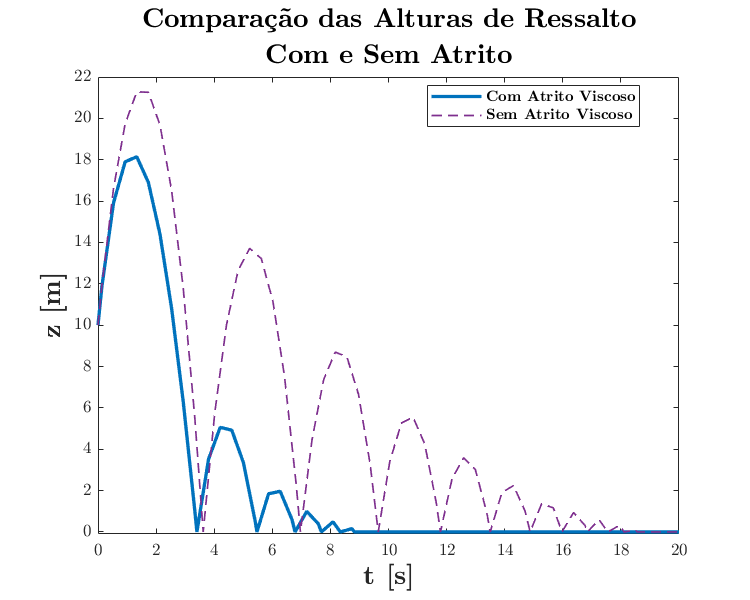
\includegraphics[width=0.6\textwidth]{img/P2/P2-compareTrajetorias.png}
    \caption{Altura de ressalto com efeito do atrito a \textcolor{blue}{azul}.}
    \label{fig:CompareAtrito}
\end{wrapfigure}

\vphantom{123}
\vskip -0.75em
\vphantom{123}

\noindent $\pmb{\rightarrow}$ \textit{\textbf{Observações}}
\\[6pt]
\hspace*{1.2em}$\blacktriangle$ É verificada uma redução da altura máxima que a bola atinge após cada ressalto, face ao exemplo isento de atrito. O fenómeno de Zeno (\textit{vide} \hyperref[subsec:P1]{sec- ção P1})  é também atingido mais rapidamente em relação ao modelo anterior.
\\[6pt]
Esta realidade é trivialmente explicada pela mecânica subja- cente ao problema:

\vskip 3.5em
\noindent $\pmb{\rightarrow}$ \textit{\textbf{Movimento de queda}}

\noindent Reconhecendo que $\dot v_{z_0} = -g \approx -9.81$ ms$^{-2}$, verifica-se um acréscimo de velocidade, subsequentemente verifica-se um acréscimo de \textit{drag} e um decréscimo da \textit{net force}. Por sua vez o decréscimo da \textit{net force} implica uma redução da velocidade. Deduz-se então que a velocidade continua a crescer, mas cada vez mais lentamente: \underline{A velocidade de impacto é menor na presença de \textit{drag}}.

\vspace{1em}
\noindent $\pmb{\rightarrow}$ \textit{\textbf{Movimento de subida após ressalto}}

\noindent Na subida, para além da velocidade após impacto ser reduzida graças ao efeito de \textit{drag} (a velocidade após impacto é dependente da anterior, \textit{vide} \hyperref[sec:intro]{secção introdutória}), a diminuição da mesma até atingir $v_{z} = 0$ ms$^{-1}$ (onde $z$ atinge $z_\textit{máx}$) é mais veloz, graças à ação da aceleração: ambas as componentes da \textit{net force} apontam na mesma direção (contrária ao movimento): \underline{A altura máxima que a bola atinge após cada ressalto é inferior}.

\clearpage
\noindent $\pmb{\rightarrow}$ \textit{\textbf{Caso Limite: Velocidade Terminal}}

\noindent A velocidade terminal (velocidade constante de queda) é atingida quando $\dot{v}_{z_0} = 0$, consequência da anulação da \textit{net force} onde $F_{drag} = F_g$:
\begin{quote}
    \textit{``Speed continues to increase, but so too does drag. As drag increases, acceleration decreases. Eventually one can imagine a state when the drag and weight forces are equal. You are in equilibrium.''}\cite{elert}
\end{quote}

\noindent Simulando a queda livre da bola\footnotemark[11] de $z_0 = 100$ m e para $\alpha = 1$, o efeito do atrito viscoso, já previamente discutido, é evidente:
\begin{figure}[H]
    \centering
    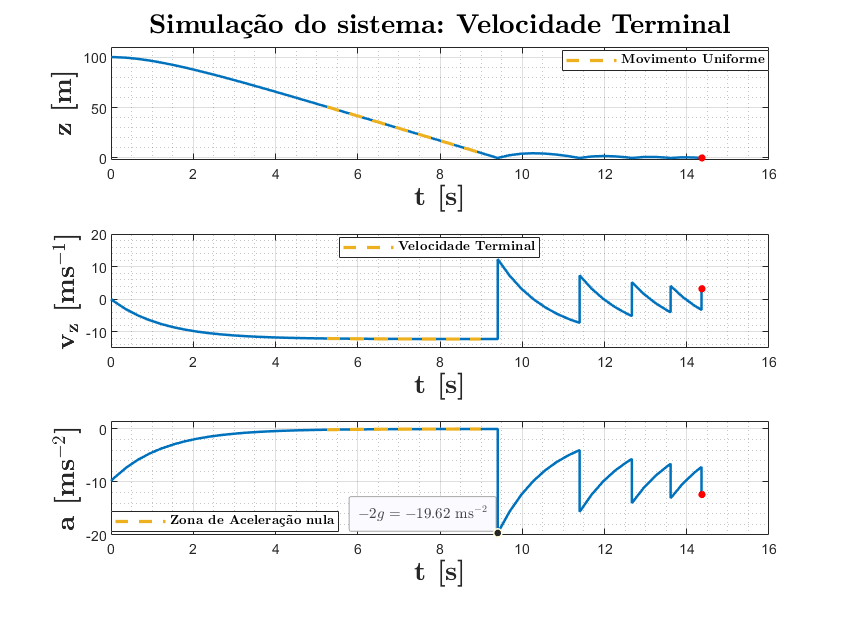
\includegraphics[width = 0.9\linewidth]{img/P2/P2-VelocidadeTerminal.png}
    \caption{Efeito do atrito na aceleração e na velocidade, alcançando a velocidade terminal. O marcador (\textcolor{red}{$\bullet$}) denota o fim da simulação.}
    \label{fig:TerminalVelocity}
\end{figure}

\footnotetext[11]{Em mecânica clássica, a queda livre é o movimento resultante \underline{unicamente} da aceleração provocada pela gravidade (i.e., $v_{z_0} = 0$ ms$^{-1}$).}

\definecolor{MnBlue}{RGB}{60, 79, 118}
\definecolor{LavenderWeb}{RGB}{221, 219, 241}
\setlength\fboxrule{1.5pt}
\hspace*{-1.5em}\fcolorbox{MnBlue}{LavenderWeb}{%
    \minipage[t]{\dimexpr1\linewidth-2\fboxsep-2\fboxrule\relax}
        \noindent $\pmb{\rightarrow}$ \textit{\textbf{Curiosidade}}
        \\
        A aceleração após o impacto é:
        
        \vspace{-0.5em}
        $$
            m\dot v_z = - F_a - mg \implies \dot v_z = - \dfrac{F_{drag}}{m} - g
        $$
        
        \vspace{-0.5em}
        Como a bola atinge a velocidade terminal, sabe-se que:
        $$
            F_{drag} = F_g \implies F_{drag} = mg\; \rightarrow\; \dfrac{F_{drag}}{m} = g
        $$
        
        \vspace{-0.5em}
        Finalmente, resolvendo em ordem a $\dot{v}_z(t_1^+)$, obtém-se:
        $$
            \therefore \dot v_z(t_1^+) = - 2g \rightarrow -19.62 \text{ ms}^{-2}
        $$

        \vspace{-0.5em}
        \hfill\ensuremath{\Box}
    \endminipage}
%//==============================--@--==============================//%